\subsection{Challenges}
\label{subsec:interconnect-sc-store-ops-challenges}


\subsubsection{Determining the right PCIe resource and instruction combination}

Of the transaction types outlined in \Cref{tab:pcie-transaction-types}, a software application can only generate a configuration or memory read and write on a modern system that only has PCIe devices
\footnote{I/O reads and writes may be available if a legacy PCI device is attached.
Messages and Completions are not controlled by the software application and, hence, can not be generated directly.}.
However, it is sufficient to explore only memory reads and writes as possible transactions since memory reads and configuration reads and writes are all non-posted transactions and will follow the same ordering rules.

We use a program that follows the pseudocode outlined in \Cref{lst:pcie-mem-reads-v-writes}
\footnote{\textit{mfence} on AMD CPUs is fully serialising and ensures all instructions, not just memory operations, finish before the barrier.}
to profile for the execution time of \textit{load} and \textit{store} instructions.
As we can see in \Cref{fig:pcie-mem-reads-v-writes}, the execution time of memory loads (and hence non-posted transactions) increases linearly with the number of memory loads issued.
This is because a load operation has to wait for a previous load operation to complete 
\footnote{While this is not enforced by PCIe ordering rules, it may be enforced by the PCIe controller implementation}.
This hampers the attacker's ability to always have one pending packet in the PCIe controller, which can only be delayed by the victim's traffic.
However, that is not the case for memory stores, and as such, we determine that memory stores are the correct type of transaction for the attacker.

\begin{minipage}{\textwidth}
\lstinputlisting[language=Python]{code/interconnect-sc/pcie-mem-reads-v-writes.py}
\captionsetup{type=lstlisting}
\caption{Pseudo-code for profiling of the execution time of load and store instruction on PCIe memory}
\label{lst:pcie-mem-reads-v-writes}
\end{minipage}


\begin{figure}[!htb]
    \centering
    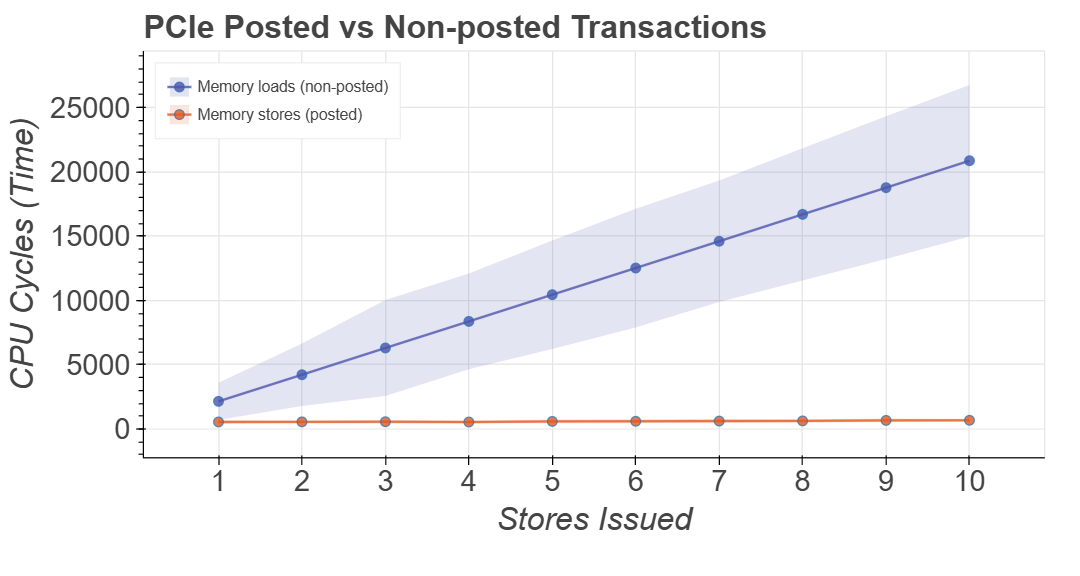
\includegraphics[width=\columnwidth]{figures/interconnect-sc/pcie_mem_reads_v_writes.png}
    \caption{Comparison: PCIe memory reads vs writes}
    \label{fig:pcie-mem-reads-v-writes}
\end{figure}

\subsubsection{Issuing and timing a continuous stream of store instructions}
\label{subsubsec:interconnect-sc-store-ops-challenges-measuring-time}

The code in \Cref{lst:pcie-mem-reads-v-writes} contains an \textit{mfence} instruction, which ensures that the \textit{store} operations before the instruction have been completed before the \textit{mfence} instruction completes.
However, this prohibits the attacker from having a continuous, steady stream of \textit{store} operations (which helps ensure that there is always one pending packet in the PCIe controller).
Simply removing the \textit{mfence} from the code is not sufficient, as then the end timer may execute out-of-order with respect to the issued stores, giving a false execution time.
To fix this, the attacker needs a mechanism that can issue as many \textit{store} instructions as possible while having the ability to time the completions at the level of each instruction.

As discussed in \Cref{subsec:interconnect-sc-background-cpu-arch}, the CPU cores have a fixed capacity of 24 instructions per scheduler and an additional 64 stores capacity in the load-store unit (LSU).
Any instruction that is not yet in the schedulers can not be executed out-of-order until it gets a slot in the scheduler.
We leverage this behaviour of the CPU to develop a mechanism that can issue multiple \textit{store} instructions while having the ability to time individual completions.

If we issue $N$ \textit{store} instructions, which can completely fill the \textit{store} unit and the schedulers, the next instruction will have to wait until one of the previously issued \textit{store} operations have been completed.
As the AMD CPU can issue 2 stores per cycle, it can issue $N = 3 * 24 + 64 = 136$ instructions in 68 cycles, which is an order of magnitude less than the time to complete one store (see \Cref{fig:pcie-mem-reads-v-writes}).
This guarantees that no \textit{store} instruction would be completed before the entire store unit and all the scheduler slots are filled.
Any instruction issued after the $N$ stores will not be executed until one of the stores finishes.
Hence, follow with a continuous stream of $timer...store$ pairs, where the timer gets executed out of order as soon as one of the previous stores retires, and the \textit{store} fills up the empty scheduler slot again, blocking the next $timer...store$ pair.
We outline the pseudo-code for this algorithm in \Cref{lst:measuring-time}.
\Cref{fig:loremipsum} shows the outcome of running this algorithm for various $N$ values. 
As we can see, the measured time difference changes more after reaching a threshold value.

\begin{minipage}{\textwidth}
\lstinputlisting[language=Python]{code/interconnect-sc/measuring-time.py}
\captionsetup{type=lstlisting}
\caption{Pseudo-code for measuring time of individual stores while issuing multiple stores in parallel}
\label{lst:measuring-time}
\end{minipage}

\subsubsection{Reverse Engineering the CPU architecture}
\label{subsubsec:interconnect-sc-store-ops-challenges-reverse-engineering}


\subsubsection{Microcode Updates}
\label{subsubsec:interconnect-sc-store-ops-challenges-microcode-updates}